%!TEX root = thesis.tex

\chapter{Research Framework} % (fold)
\label{cha:research_framework}
In order to examine a possible relation between stack traces and priority, severity and time-to-fix, a research framework is used to investigate the hypotheses described in Section~\ref{sec:research_questions}. This chapter describes this research framework, where the next chapter discusses how the framework is used to analyse the actual data.

\section{Overview} % (fold)
The research framework, as depicted in Figure~\ref{fig:research_framework} consists of four major parts:

\begin{enumerate}
	\item Source code extraction (Section \ref{sec:source_code_extraction})
	\item Issue report extraction (Section \ref{sub:issue_report_extraction})
	\item Stack trace matching (Section \ref{sec:stack_trace_extraction_and_mapping})
	\item Data analysis (Chapter \ref{cha:data_analysis})
\end{enumerate}

\begin{figure}[!ht]
	\centering
		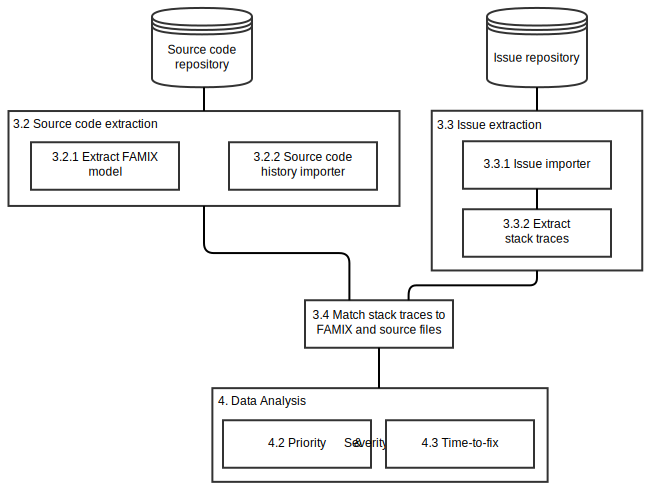
\includegraphics[width=1\textwidth]{img/research_framework.pdf}
	\caption{Overview of the research framework.}
	\label{fig:research_framework}
\end{figure}

The data extraction part makes sure both the source code repository as well as the issue report repository are available for querying. All extractions are performed using the Evolizer framework \cite{Gall2009}, which is a plugin for the Eclipse IDE. Evolizer is a platform for mining software artifact repositories into models. Also, Evolizer is extended to support stack trace extraction and matching. The source code for this extension is available.

The source code extraction consists of generating a model of the source code and the source code repository. The issue reports are extracted from the issue repository into another model, after which stack traces are extracted from these issues. Finally, both the source code model, the source code repository model and the issue model are linked. Based on this data set, the analysis of Chapter \ref{cha:data_analysis} can be performed. In this analysis, two low-level metrics are used: lines of code, and time-to-fix. Both metrics are discussed in Section \ref{sec:low_level_metrics}.

% section overview (end)
\section{Source code extraction} % (fold)
\label{sec:source_code_extraction}
The source code of a project under investigation is extracted from the source code repository in two ways:

\begin{enumerate}
	\item Extraction of the source code into a language independent meta-model that describes the static structure of the source code (Section~\ref{sub:famix_model_extraction})
	\item Extraction of the complete source code repository into a meta-model (Section~\ref{sub:source_code_history_importer})
\end{enumerate} 

\subsection{FAMIX model extraction} % (fold)
\label{sub:famix_model_extraction}
The FAMIX meta-model \cite{Tichelaar2000,Tichelaar2001} is a language independent representation of the static structure of the source code of a project. Figure~\ref{fig:evolizer_class_diagram} depicts the class hierarchy of the FAMIX model as implemented in Evolizer. 

\texttt{AbstractFamixObject} is the base class for FAMIX entities and associations between FAMIX entities. A FAMIX entity represents either a package, class or method. It can also represent a \texttt{FamixVariable}, which represents class attributes, local variables, and formal parameters. Relations between these entities are represented by \texttt{FamixAssociation}s, which are for example casts, invocations or inheritance between entities.

\begin{figure}[!ht]
	\centering
		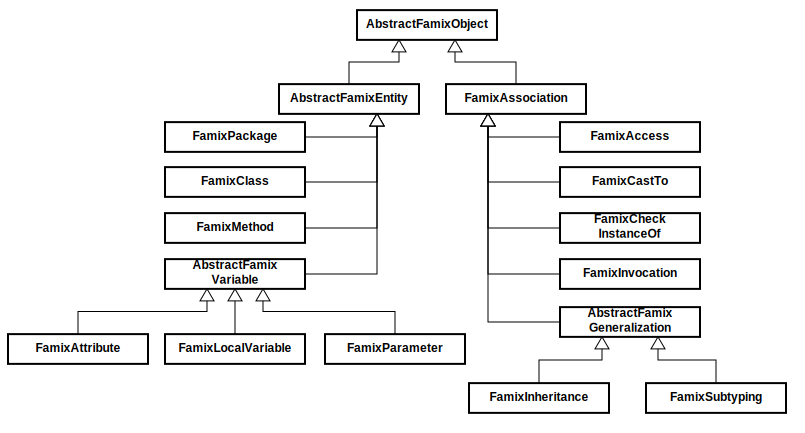
\includegraphics[width=1\textwidth]{img/FAMIX_object_model.pdf}
	\caption{Implementation of the FAMIX meta-model in Evolizer.}
	\label{fig:evolizer_class_diagram}
\end{figure}

Evolizer is able to extract a FAMIX meta-model from the source code of an Eclipse Java project. Eclipse core libraries (for example \texttt{org.eclipse.jdt.core}) are used to extract the FAMIX model. The extracted model is saved in the Evolizer relational database, where it can be queried using the Evolizer Hibernate\footnote{\url{http://www.hibernate.org/}} model or via plain SQL queries. 

Evolizer also offers several metrics, such as number of methods of a class, lines of code of a class, or cyclomatic complexity \cite{McCabe1976}. For some metrics, such as lines of code, it is necessary to have a model of the actual source files, which are part of the source code history. The extraction of this model is detailed in Section~\ref{sub:source_code_history_importer}.
% subsubsection famix_model_extraction (end)

\subsection{Source code history importer} % (fold)
\label{sub:source_code_history_importer}
The source code repository is also extracted to a meta-model, containing versioned files, revisions, branches, releases, et cetera \cite{Fischer}. Figure~\ref{fig:source_code_repository_metamodel} shows a simplified depiction of the source code history meta-model. Central in this model is a \texttt{VersionedFile}, which is a specialised implementation of \texttt{File} that is, of course, versioned. Each versioned file has one or more revisions. A revision is linked to the source code content for that specific revision. The modification report states the commit message for that revision. As can be seen, the meta-model for the source code repository is heavily inspired by CVS like SCM systems. 

\begin{figure}[!ht]
	\centering
		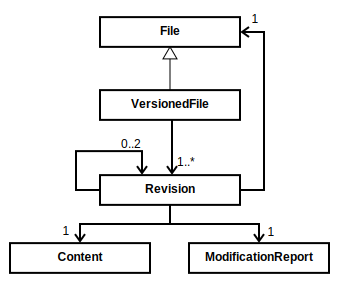
\includegraphics[width=0.5\textwidth]{img/version_history_model.pdf}
	\caption{Source code repository history meta-model.}
	\label{fig:source_code_repository_metamodel}
\end{figure}

Evolizer imports a complete source code repository history into its database, including the contents of all file revisions. In the case of a CVS repository, at first the complete log file is parsed. In this stage, all files under version control are recognized, including all their revisions. After this, the source code contents for all file revisions are read and put into the database, completing the model.
% subsubsection source_code_history_importer (end)
 
% subsection source_code_extraction (end)

\section{Issue report extraction} % (fold)
\label{sub:issue_report_extraction}
Next to the source code repository, Evolizer is also used to extract the issue repository. After the complete repository is extracted, all issue comments are examined for stack traces.

\subsection{Issue repository importer} % (fold)
\label{sub:issue_importer}
Figure~\ref{fig:issue_repo_metamodel} shows a partial representation of the issue meta-model. Each bug repository is split into several levels, starting at a global classification, down to products and specific components of that products. An issue has several properties, such as status, priority, severity and assigned milestone. Each issue can have several comments that form the discussion for that bug report. Also, the history of a bug, such as fixing or closing a bug, (re)assigning a developer, changing priority, et cetera, is captured as activities. 

\begin{figure}[!ht]
	\centering
		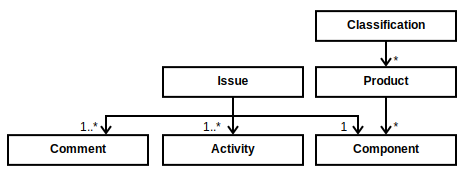
\includegraphics[width=0.7\textwidth]{img/issue-model.pdf}
	\caption{Issue repository meta-model.}
	\label{fig:issue_repo_metamodel}
\end{figure}

Evolizer is able to convert Bugzilla bug repositories to this meta-model. It is possible to extract a complete bug repository or a specific range of bug reports. In order to only extract certain bug reports, for example for a specific product only, Evolizer was extended to be able to enter a comma separated list of bug IDs to import. All bugs are read from Bugzilla in a XML format and parsed by Evolizer using a SAX2\footnote{\url{http://www.saxproject.org/}} parser. After this, the activities of a bug report are parsed. These activities are only available in HTML format, so a HTML parser was used to extract this information.

\subsubsection{Issues} % (fold)
When parsing Bugzilla data using the XML parser, several issues were found\footnote{See Appendix~\ref{cha:bugzilla_importer_xml_parser_issues} for more details.}. These issues were mitigated by correctly implementing the XML importer. Also, some other bugs in the state machine were fixed, such as validating the Bugzilla XML to the correct Document Type Definition. Finally, functionality was added to import bug reports multiple times, without resulting in duplicate data in the Evolizer database.
% paragraph issues (end)
% subsubsection issue_importer (end)

\subsection{Stack trace extraction} % (fold)
\label{sub:stack_trace_extraction}
After all bug report comments are imported, a subsequent pass is performed in order to extract all stack traces from these comments. A stack trace consists of a number of stack trace frames, which are represented by lines in a stack trace. A typical Java stack trace looks like this:

{\small
\begin{verbatim}
	java.lang.ArrayIndexOutOfBoundsException: 2048 	
	at org.eclipse.jdt.internal.core.DiskIndex.readStreamInt(DiskIndex.java:48)
	at org.eclipse.jdt.internal.core.DiskIndex.readHeader(DiskIndex.java:779)
	at org.eclipse.jdt.internal.core.DiskIndex.initialize(DiskIndex.java:379)
	...
	at org.eclipse.core.internal.jobs.Worker.run(Worker.java:48)
\end{verbatim}
}

Complete stack traces are extracted from bug report comments using a regular expression matching on `...Exception' and multiple parts starting with `at' (representing the stack frames):

{\small
\begin{verbatim}
	(.+Exception[^\\n]+(\\s+at\\s?.+)+)+
\end{verbatim}
}

\begin{sloppypar}
Each stack trace frame consists of a qualified name (\texttt{org.eclipse.jdt.internal.core.DiskIndex.readStreamInt}), a source file (\texttt{DiskIndex.java}) and a line number (48)\footnote{\url{http://docs.oracle.com/javase/1.5.0/docs/api/java/lang/StackTraceElement.html}}. The qualified name can subsequently be split into a package name, class name and a method name. 
\end{sloppypar}

Each stack trace frame was parsed using the following regular expression:
{\small
\begin{verbatim}
	((([a-zA-Z0-9\\$]+)\\.)*)(([a-zA-Z0-9\\$]+)\\.([a-zA-Z0-9\\$]+))(\\((.+):(.+)\\))
\end{verbatim}
}

In order to mine all stack traces, first all complete stack traces are extracted from the already imported bug reports. Each bug report can have multiple comments, which in turn can have multiple stack traces. After this, a subsequent pass is performed to parse all stack trace call stacks, again using a regular expression. Each stack trace frame is split into a package name, class name, method name, file name and line number.

\begin{figure}[!ht]
	\centering
		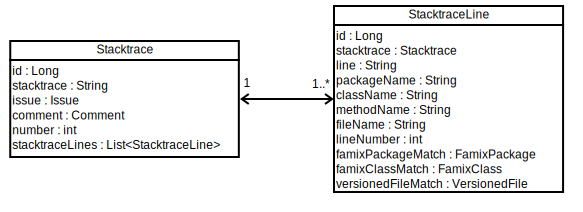
\includegraphics[width=0.8\textwidth]{img/stacktracemodel.pdf}
	\caption{Stack trace model class diagram.}
	\label{fig:stacktrace_model}
\end{figure}

In order to be able to parse and persist all stack traces and corresponding stack frames from the bug repository, Evolizer and its associated object model have been extended. The corresponding class diagram is shown in Figure~\ref{fig:stacktrace_model}.
% subsubsection stack_trace_extraction (end)

% subsection issue_report_extraction (end)

\section{Stack trace extraction and mapping} % (fold)
\label{sec:stack_trace_extraction_and_mapping}
In this stage of data gathering, a FAMIX meta-model, source code repository meta-model, and an issue repository meta-model extended with stack traces are  available. Using the stack traces found, all these models can be linked. For this, each stack trace line will be matched with a FAMIX package, FAMIX class and a versioned file. The resulting overall model is depicted in Figure~\ref{fig:complete_meta_model}.

\begin{figure}[!ht]
	\centering
		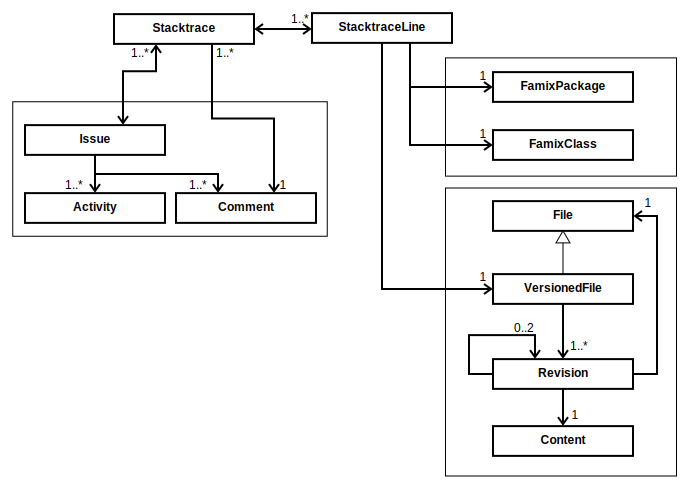
\includegraphics[width=1\textwidth]{img/linked_meta_model.pdf}
	\caption{Complete meta-model for the research framework.}
	\label{fig:complete_meta_model}
\end{figure}

\begin{sloppypar}
FAMIX packages and classes are matched based on string equality. For \texttt{VersionedFile}s, the package and file name from the stack trace line are used to (partly) represent the file path. For example, a package \texttt{org.eclipse.jdt.internal.core} and file name \texttt{DiskIndex.java} is converted to the file path \texttt{org/eclipse/jdt/internal/core/DiskIndex.java}, which in turn is matched to the available \texttt{VersionedFile}s.
\end{sloppypar}

This concludes the extraction of a complete meta-model from the bug report repository and the source code repository, using stack traces to match both models.
% section stack_trace_extraction_and_mapping (end)

\section{Low-level metrics} % (fold)
\label{sec:low_level_metrics}
The metrics used in Chapter \ref{cha:data_analysis} are: lines of code and time-to-fix. This section gives a definition of both these metrics.

\subsection{Lines of code} % (fold)
In order to determine the lines of code of a source file, only the lines which contain actual source code are counted. Comments, import statements, package declarations and empty lines are ignored.

\subsection{Time-to-fix} % (fold)
\label{sub:time_to_fix}
Only issue reports that have resolution \textsc{fixed} and status \textsc{verified} are considered to be fixed, and hence have a time-to-fix. Each bug has an activity history, which records changes in bug properties. The time-to-fix is the number of days between the creation date of the issue report and the \emph{latest} activity in which the resolution changed to `fixed'. This way, possible incomplete fixes are ignored.
% subsection time_to_fix (end)
% section low_level_metrics (end)

% chapter research_framework (end)
